\documentclass[hyperref={pdfpagelabels=false},aspectratio=34,14pt]{beamer}
\usepackage{lmodern} %TODO: descobrir o que mudou as fontes dos slides (comparar com os primeiros)
\usepackage[utf8]{inputenc}
\usepackage[T1]{fontenc}
\usefonttheme[onlymath]{serif}
\usepackage[brazil]{babel}
\usepackage[outputdir=..]{minted}
\usepackage{xcolor}
\usepackage{soul} % strikethrough
\usepackage{advdate}
\usepackage{graphicx}
\usepackage[ampersand]{easylist}
\usepackage{multirow}
\usepackage{tikz}
\usetikzlibrary{shapes,arrows,positioning}
\usetikzlibrary{circuits.logic.US}
\usetikzlibrary{matrix,calc}
\usepackage{karnaugh-map}

\usepackage{pgfpages}
\setbeamertemplate{note page}{\pagecolor{yellow!5}\insertnote}\usepackage{palatino}
\newcommand{\yes}{edge node [above] {yes}}
\newcommand{\no}{edge  node [left]  {no}}
\newcommand{\textttb}[1]{\textcolor{blue}{\ttfamily #1}}

% \setmathfont{Latin Modern Math}[version=lm]

\graphicspath{{../figs/}}

\definecolor{bgc}{rgb}{0.95,0.9,0.95}
\definecolor{links}{HTML}{2A7F7F}
\hypersetup{colorlinks,linkcolor=,urlcolor=links}

\newminted{verilog}{fontsize=\scriptsize, 
		   linenos,
		   numbersep=8pt,
           bgcolor=bgc,
           tabsize=4,
		   framesep=3mm} 
%		   frame=lines,

\newcommand{\verilog}[1]{\verilogf{#1}{\footnotesize}

\newcommand{\verilogf}[2]{\inputminted[fontsize=#2, 
		   linenos,
		   tabsize=2,
		   numbersep=4pt,
           bgcolor=bgc,
		   framesep=3mm]{verilog}{../codes/#1.v}
}

\newminted{nasm}{fontsize=\scriptsize, 
		   linenos,
		   numbersep=8pt,
           bgcolor=bgc,
		   framesep=3mm} 

% \author[shortname]{\scriptsize Prof. Edilson Kato \and Prof. Maurício Figueiredo \and Prof. Ricardo Menotti\newline
% \href{mailto:kato@ufscar.br}{kato@ufscar.br} \and    \href{mailto:mauricio@ufscar.br}{mauricio@ufscar.br} \and
% \href{mailto:menotti@ufscar.br}{menotti@ufscar.br}}

\newcommand{\newauthor}[2]{
  \parbox{0.40\textwidth}{
    \texorpdfstring
      {
        \centering
        \footnotesize #1 \newline
        {\scriptsize{\urlstyle{same}\href{mailto:#2}{#2}\urlstyle{tt}}}
      }
      {#1} \newline
  }
}

\author{
%   \newauthor{Prof. Edilson Kato}{kato@ufscar.br}
% \and
  \newauthor{Prof. Ricardo Menotti}{menotti@ufscar.br}
\and 
  \newauthor{Prof. Maurício Figueiredo}{mauricio@ufscar.br}
% \and
%   \newauthor{Prof. Roberto Inoue}{rsinoue@ufscar.br}
}

\institute{\href{http://www.dc.ufscar.br/}{Departamento de Computação} \\
           \href{http://www.ufscar.br/}{Universidade Federal de São Carlos}} 
\titlegraphic{
  \makebox[.85\paperwidth]{
    
\includegraphics[height=1cm]{figs/LogoDC} 
    \hfill 
    
\includegraphics[height=1cm]{figs/LogoUfscar}}}
\date{Atualizado em: \today} 
% \date{\DayAfter[+1]} % +/-

%\logo{
\includegraphics[height=1cm]{figs/LogoUfscar}
\includegraphics[height=1cm]{figs/LogoDC}}

\title{Lógica Digital (1001351)}

\AtBeginSubsection[]
{
  \begin{frame}<beamer>{Roteiro}
    \tableofcontents[currentsection,currentsubsection]
  \end{frame}
}

\addtobeamertemplate{navigation symbols}{}{%
    \usebeamerfont{footline}%
    \usebeamercolor[fg]{footline}%
    \hspace{1em}%
    \raisebox{1.2pt}[0pt][0pt]{\insertframenumber/\inserttotalframenumber}
}


\subtitle{Title} % 

\begin{document}

\begin{frame}
	\titlepage
\end{frame} 

% % Uncomment if you want a summary slide
% \begin{frame}{Conteúdo}
% 	\tableofcontents
% \end{frame}

% \section{Section bullets} %%%%%%% Can be used as slide title with \insertsection command

% \begin{frame}{\insertsection} % Slide with bullets
% 	\begin{itemize}
% 		\item ;
% 		\item .
%     \end{itemize}
% \end{frame}

% \begin{frame}{\insertsection: 2 levels}
%     \begin{itemize}
%         \item :
%         \begin{itemize}
%             \item ;
%             \item ; e 
%             \item ;
%         \end{itemize}  
%         \item :
%         \begin{itemize}
%             \item ;
%         \end{itemize}
%     \end{itemize}
% \end{frame}

% \section{Section picture}

% \begin{frame}{\insertsection}
%     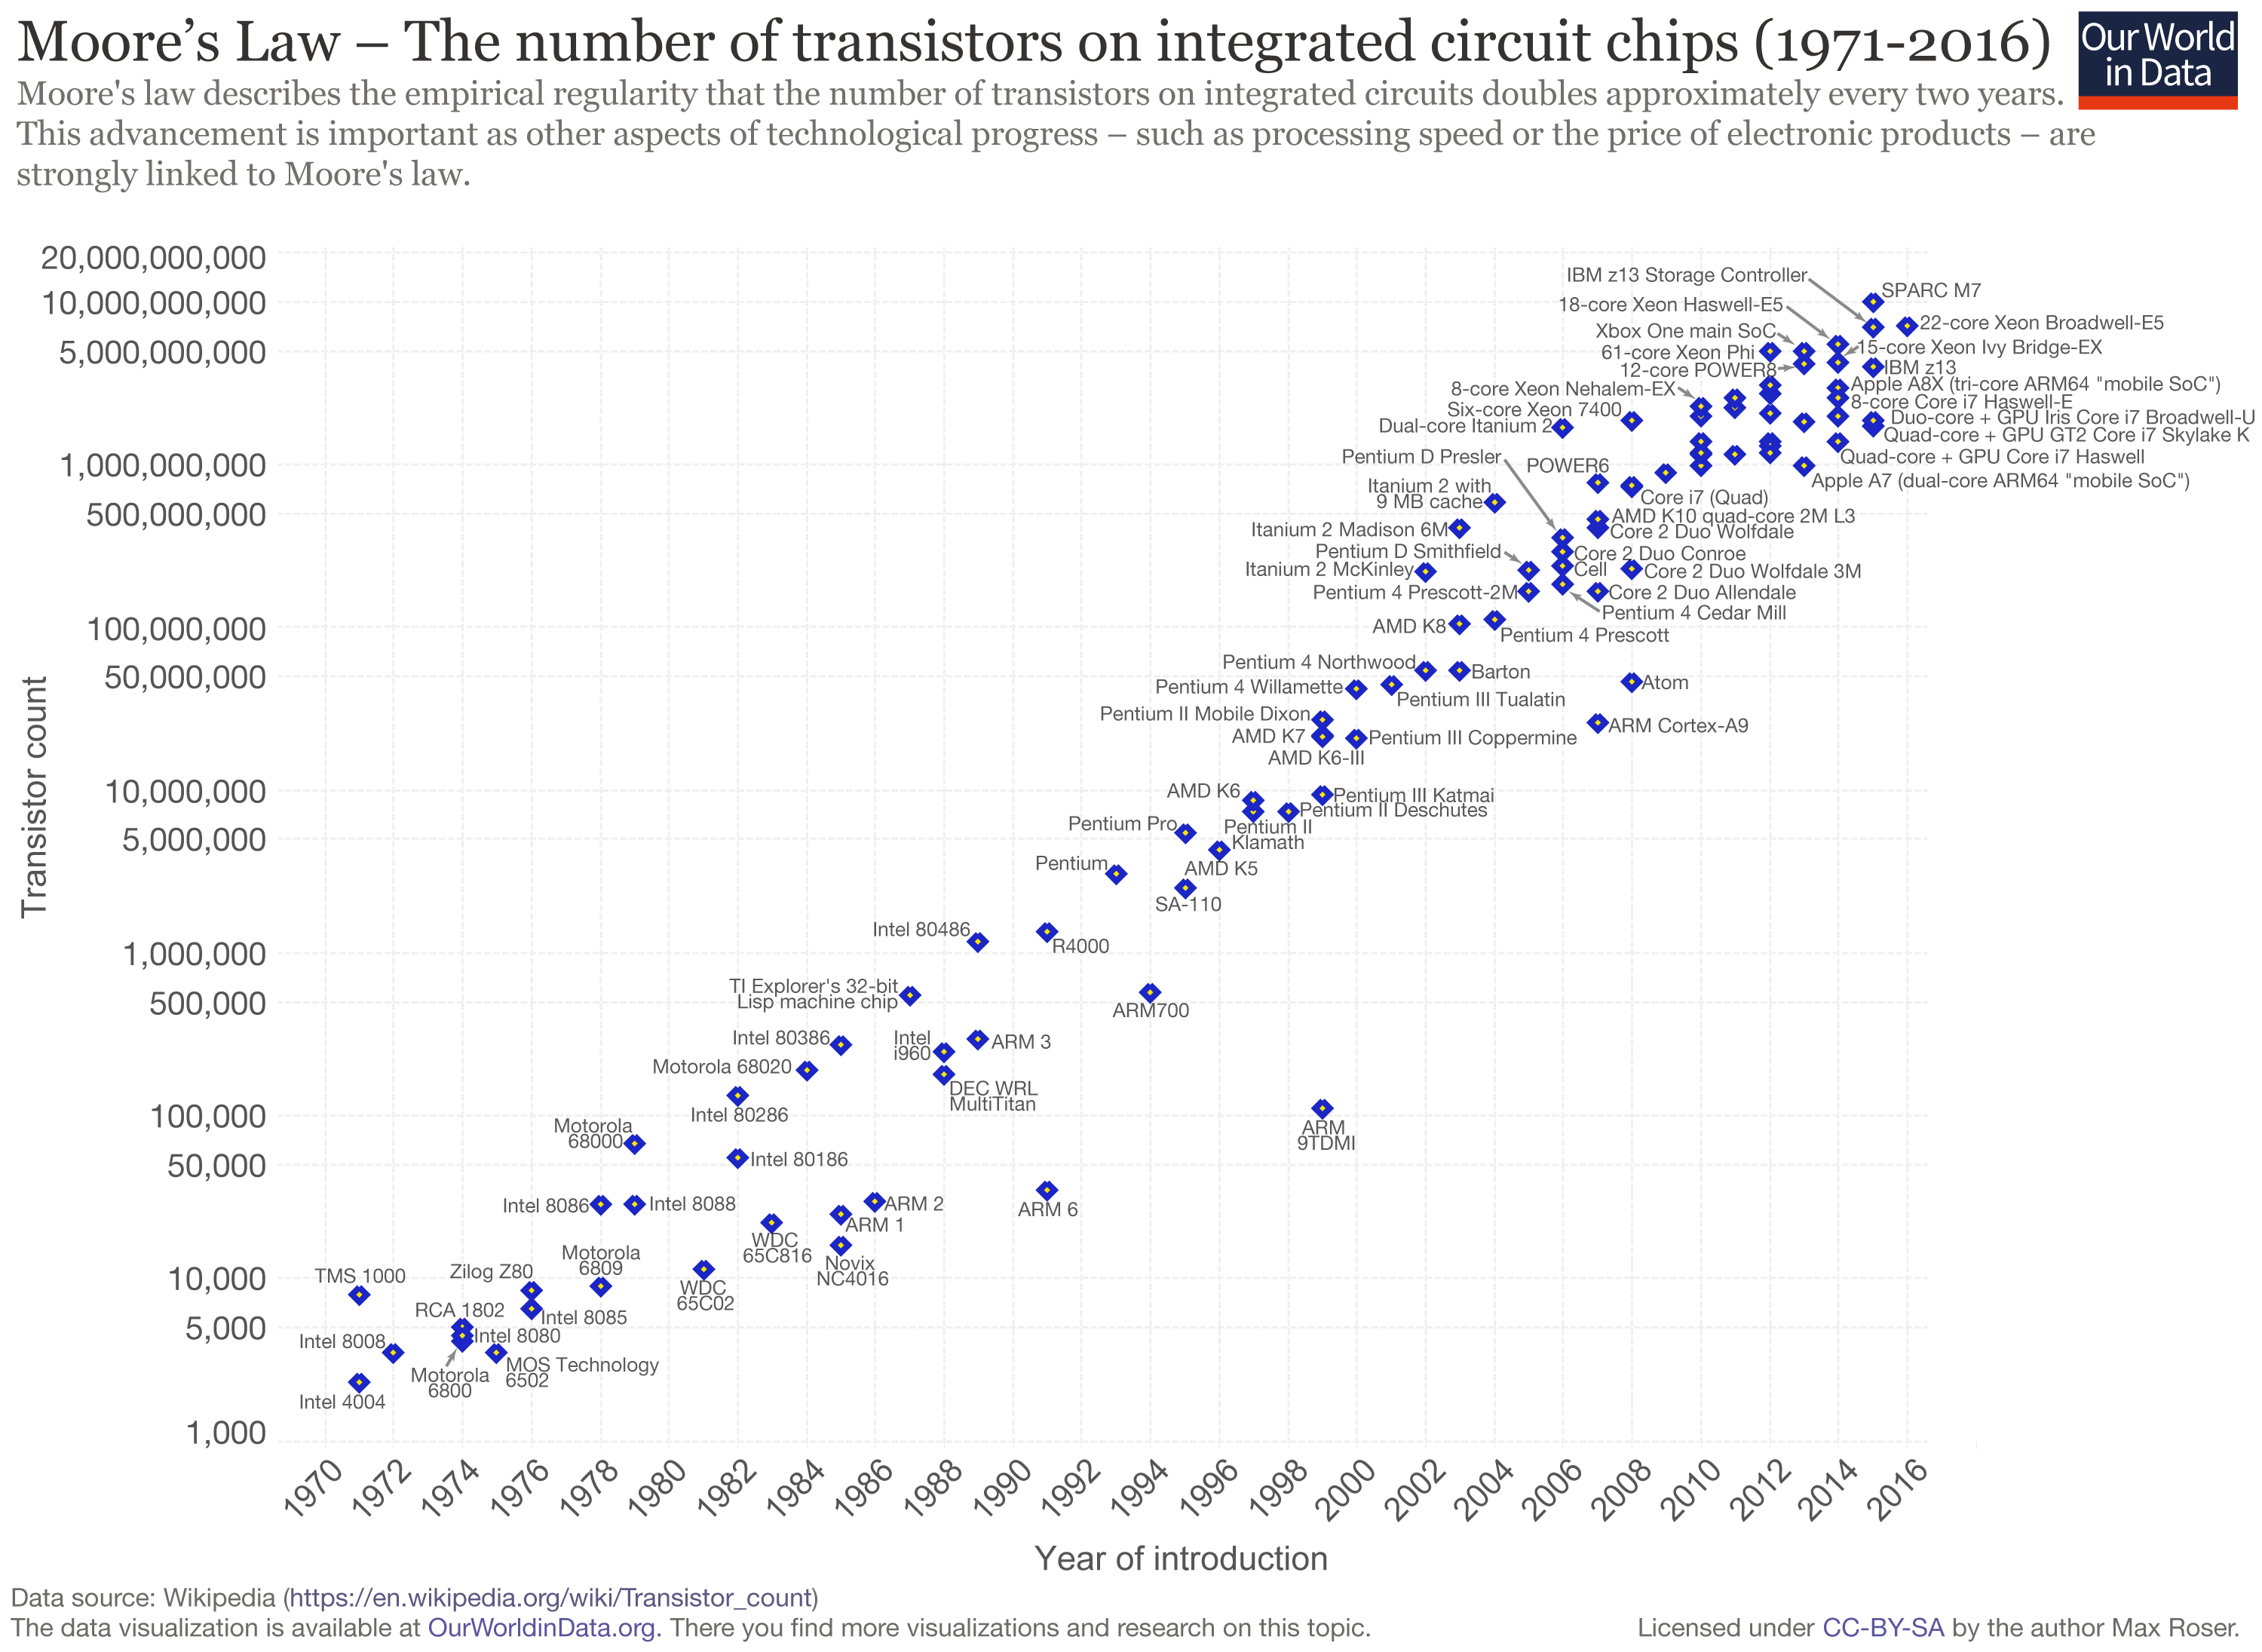
\includegraphics[width=.9\textwidth]{Moore}
% \end{frame}

% \section{Section table}

% \begin{frame}{\insertsection}
% 	\begin{itemize}
%         \item O intervalo de inteiros que pode ser representado por um número binário depende do número de bits usados: 
%     \end{itemize}
%     \vspace{-0.5cm} % to save space between text above and table below
%     \begin{table}[]
%         \centering \scriptsize 
%         \begin{tabular}{cc} % center, left or right 
%             \hline
%             \textbf{Decimal} & \textbf{Binária} \\
%             \hline
%             \hline
%              00 & 0000 \\
%              01 & 0001 \\
%              02 & 0010 \\
%              03 & 0011 \\
%             \hline
%         \end{tabular}
%     \end{table}
% \end{frame}

% \section{Code}

% \begin{frame}[fragile]{\insertsection}
% 	\begin{verilogcode}
% module fulladd (Cin, x, y, s, Cout); 
%   input Cin, x, y;
%   output s, Cout;

%   xor (s, x, y, Cin); 
%   and (z1, x, y);
%   and (z2, x, Cin); 
%   and (z3, y, Cin);
%   or (Cout, z1, z2, z3);
% endmodule
% 	\end{verilogcode} 
% \end{frame}

% \section{Section mixed}

% \begin{frame}{Alternative title to the section} 
%     \begin{columns}
%         \begin{column}{0.60\textwidth}
%             \begin{itemize}
%                 \item ;
%                 \item ;
%                 \item ;
%                 \item . 
%             \end{itemize}
%         \end{column}
%         \begin{column}{0.40\textwidth}
%             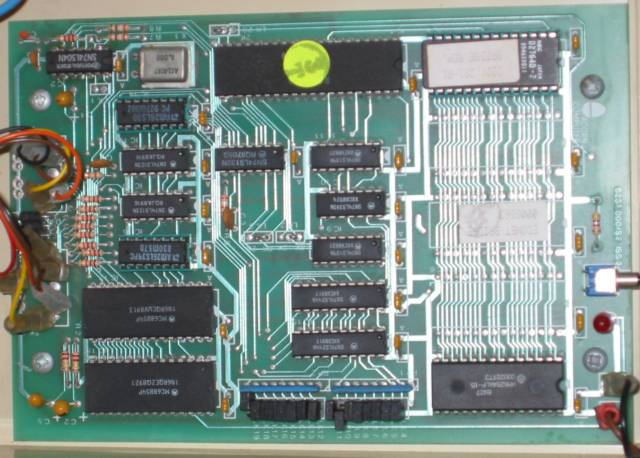
\includegraphics[angle=90,width=\textwidth]{Econet}
%         \end{column}        
%     \end{columns}
% \end{frame}

% \section{Section drawing}

% \begin{frame}{\insertsection}
%     \centering 
%     \tikzstyle{decision} = [diamond, draw, fill=red!20, text width=4.5em, text badly centered, node distance=2.3cm, inner sep=0pt]
%     \tikzstyle{block} = [rectangle, draw, fill=red!20, text width=10em, text centered, rounded corners, minimum height=2em]
%     \tikzstyle{line} = [draw, -latex']
%     \tikzstyle{cloud} = [draw, ellipse,fill=red!20, node distance=3cm,
%     minimum height=2em]
% \resizebox{0.5\textwidth}{!}{%
% \begin{tikzpicture}[node distance = 1.3cm, auto]
%     \node [cloud] (init) {Produto requerido};
%     \node [block, below of=init] (specs) {Definir espeficicação};
%     \node [block, below of=specs] (design) {Projeto inicial};
%     \node [block, below of=design] (sim) {Simulação};
%     \node [block, right=1cm of sim] (redesign) {Reprojeto};
%     \node [decision, below of=sim] (right) {Projeto correto?};
%     \node [block, below=0.7cm of right] (proto) {Prototipação};
%     \node [block, below of=proto] (test) {Testes};
%     \node [block, right=1cm of proto] (corec) {Correções};
%     \node [decision, below of=corec] (minor) {Erros menores?};
%     \node [decision, below=0.7cm of test] (meets) {Cumpre especificação?};
%     \node [cloud, below=0.3cm of meets] (finish) {Produto finalizado};
%     \path [line] (init) -- (specs);
%     \path [line] (specs) -- (design);
%     \path [line] (design) -- (sim);
%     \path [line] (sim) -- (right);
%     \path [line] (redesign) -- (sim);
%     \path [line] (right) -| (redesign) node[near start,above] {não};
%     \path [line] (right) -- (proto) node[near start,right] {sim};
%     \path [line] (proto) -- (test);
%     \path [line] (test) -- (meets);
%     \path [line] (corec) -- (proto);
%     \path [line] (minor) -- (corec) node[near start,right] {sim};
%     \path [line] (meets) -| (minor) node[near start,above] {não};
%     \path [line] (meets) -- (finish) node[near start,right] {sim};
%     \path [line] (minor.east) -- node[near start,above] {não} ++(2,0)  -- ++(0,6.95) --  (redesign.east);
% \end{tikzpicture}}
% \end{frame}

\section{Bibliografia} %%%%%%%

\begin{frame}{\insertsection} 
	\begin{itemize}
		\item \href{https://www.google.com.br/search?q=filetype\%3Apdf+Fundamentals+of+Digital+Logic+with+Verilog+Design+&oq=filetype\%3Apdf}{Brown, S. \& Vranesic, Z. - Fundamentals of Digital Logic with Verilog Design, 3rd Ed., Mc Graw Hill, 2009}
		\item \href{https://www.asciiart.eu/}{https://www.asciiart.eu/}
	\end{itemize}
\end{frame}

% \begin{frame}[allowframebreaks]{\insertsection} 
% 	\begin{itemize}
% 		\item Básica
% 		\begin{itemize}
% 			\item Patterson, D. A. \& Hennessy, J. L. - Organização e Projeto de Computadores - A Interface Hardware/Software 4ª Ed., Editora Campus, 2014 (14 exemplares na BCo)
% 			\item \href{https://www.sciencedirect.com/science/book/9780123944245}{D. M. Harris \& S. L. Harris - Digital Design and Computer Architecture 2nd Ed., Elsevier, 2012 (2 exemplares na BCo, disponível no portal da CAPES)}
% 			\item \href{https://www.google.com.br/search?q=filetype\%3Apdf+Fundamentals+of+Digital+Logic+with+Verilog+Design+&oq=filetype\%3Apdf}{Brown, S. \& Vranesic, Z. - Fundamentals of Digital Logic with Verilog Design, 3rd Ed., Mc Graw Hill, 2009 (disponível online)}
% 		\end{itemize}
% 		\framebreak
% 		\item Complementar
% 		\begin{itemize}
% 			\item Tanenbaum, A. S. - Organização Estruturada de Computadores 5ª Ed., Pearson: Prentice-Hall, 2007
% 			\item Hamblen, J. O. et al. - Rapid Prototyping of Digital Systems SOPC Edition, Springer, 2008
% 			\item Stallings, W. - Arquitetura e Organização de Computadores, Pearson, 2010
% 			\item \href{https://www.asciiart.eu/}{https://www.asciiart.eu/}
% 		\end{itemize}
% 	\end{itemize}
% \end{frame}

\begin{frame}
	\titlepage
\end{frame} 

\end{document}